% Chapter Template

\chapter{Results} % Main chapter title

\label{Chapter4} % Change X to a consecutive number; for referencing this chapter elsewhere, use \ref{ChapterX}

%----------------------------------------------------------------------------------------
%	SECTION 1
%----------------------------------------------------------------------------------------
In this chapter, we present the experimental data recovered through the differents 
steps described in the Chapter before. Most the following results consists in 
2-D arrays representing a matrix, where in each position a color is painted, depending
on how many photons were detected in single or coincidences counts.
As we have seen, before making a Two-photon image, there are some process 
that have to be made. The first thing to do is to achieve a Gaussian behavior 
of the original diode laser. For doing so, we have to look at the beam propagation after 
the Spatial Filter. 

\section{Achiving a Gaussian Beam}

From Eq. \ref{eq:wa} we expect that the pump waist doesn't change too much with the distance
traveled, for this reason we started by measuring the spatial profile of our pump beam in different 
distances from the spatial filter. Figure \ref{fig:pro} shows the behaviour of the waist while we move away from the spatial filter.
From the Figure we can observe that the waist doesn't change significantly, if we take a closer look in the x-axis, the total separation from the 
spatial filter ($\sim100cm$)  its considerably bigger than the little change in the pump waist($\sim 100 \mu m$). There are 3 diferent lines in 
both Figures, the blue one corresponds to the pump waist at the 13.5\% of the intensity, the red one to the 50\% and the green one to the 80\%.


\begin{figure}[h!]
\centering
{  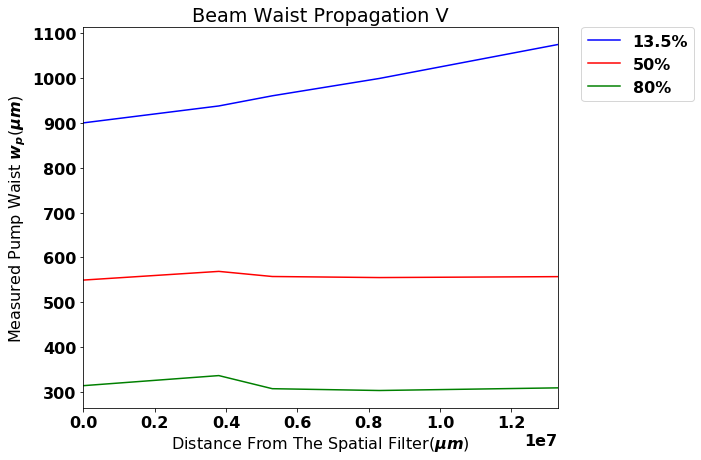
\includegraphics[width=0.45\textwidth]{Figures/propagationV.png} }
{  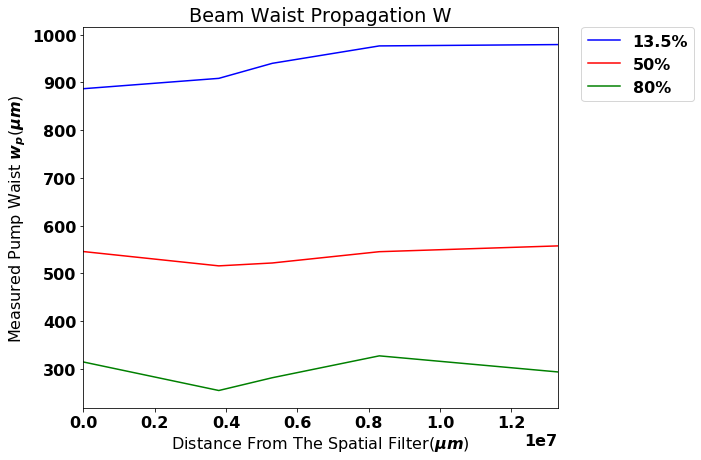
\includegraphics[width=0.45\textwidth]{Figures/propagationW.png} }
\caption{Propagation of the pump Beam, the graph shows how the $w_p$ changes with distance}
 \label{fig:pro}
\end{figure}

Figure \ref{fig:p} shows the waist measured in the V and W direction, this waist correspond to the 13.5\% of intensity. Using \ref{eq:wa}
we can make a fit to the experimental data. We observe that in the V direction the behaviour is closer 
to the one expected by theory for a gaussian beam, the blue line shows how the pump waist should change for a gaussian beam with origin point
at z=0.


\begin{figure}[h!]
\centering
{  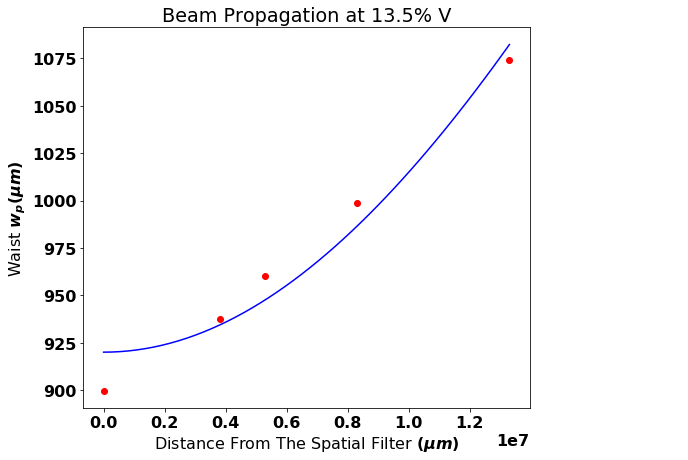
\includegraphics[width=0.48\textwidth]{Figures/proV.png} }
{  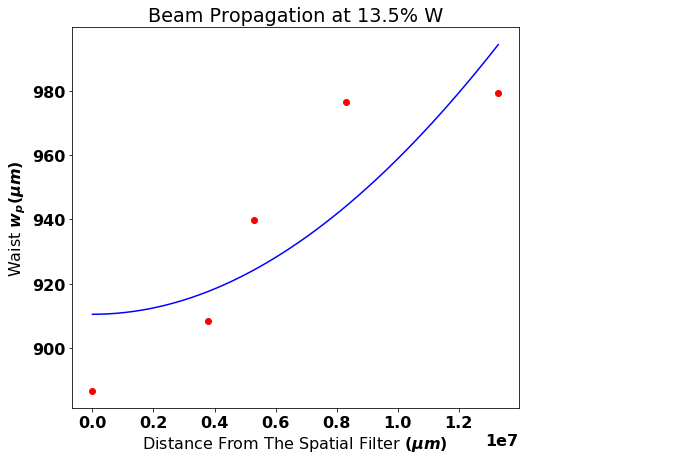
\includegraphics[width=0.48\textwidth]{Figures/proW.png} }
\caption{Fit for the change in the $w_p$ with distance, at 13.5\% intensity}
 \label{fig:p}
\end{figure}

\section{Finding The Correlated Photons}

After obtaining a Gaussian propagation, and messuring waist that no varies to much
while propagates, we focused the laser at the BBO crystal and with the help of the \textit{waist lens}
we set the $w_p=91 \mu m$. Before observing the spatial correlations of the down converted
photons, we make sure we are seing them. Figure \ref{fig:correlatedPhotonSpot} shows 
two different images recovered, where in Fig.\ref{fig:correlatedPhotonSpot}(a) we found
out that there is some problems with the alignment of the optical elements.



\begin{figure}[h!]
\centering
{  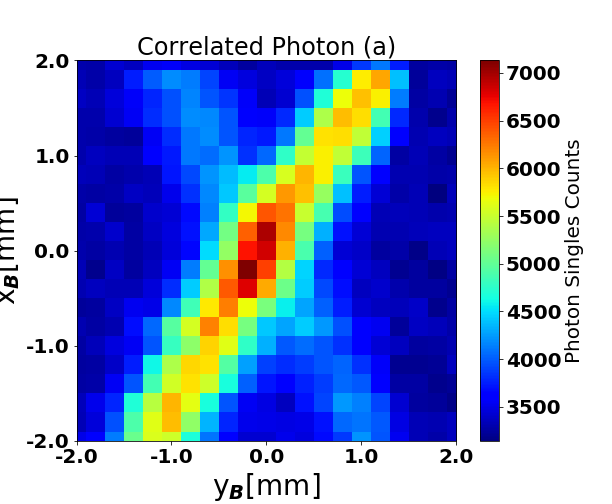
\includegraphics[width=0.48\textwidth]{Figures/correlatedPhotonSpot1.png} }
{  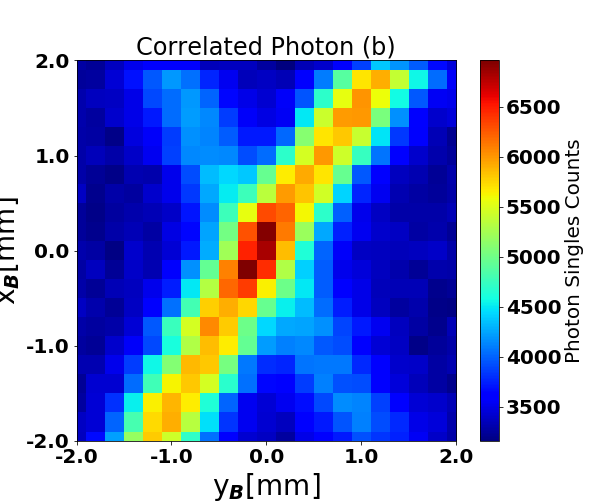
\includegraphics[width=0.48\textwidth]{Figures/correlatedPhotonSpot2.png} }
\caption{(a) and (b) shows the B-photon of the down converted pair. In (b) we moved away the translational mount of the mask}
 \label{fig:correlatedPhotonSpot}
\end{figure}

In Figure \ref{fig:correlatedPhotonSpot}(b) we can see the B-photon, and now there is
no interference caused by the bad alignment. As said before we placed a pair of polarisers
in order to filter them. In the figure we can see that just one direction of the 
down converted pair of photons,  while the other is partially filtered.


\section{Experimental Correlations }

After being sure of observing the correlated photons, we would like to observe the shape of the spatial correlations the pair of down converted
photons and see the experimental behaviour of $|\tilde{\Phi}(\vec{q}_B,\vec{q}_A)|$.
When remembering the definition of $\vec{q}_n$, it is a 2-D vector, containing the information
of the photon in x and y direction. It is clear that when counting the two photons, we have 
4 differents correlations for the pair of photons, in this monograh we focus on the correlations on the type XX and YY.There
is important to point out that this transverse momentum $\vec{q}_n$ is related with
his equivalent $\vec{r}_n$ the position of the photon, with n making reference to the A and B paths.





In Figure \ref{fig:expCorrelations} there are the correlations in the xx and yy  direction.
The 2-D matrix in Figure \ref{fig:expCorrelations}(\textit{XX Correlation}) is
 the result of repeating this recipe: placing the $D_A$ at a fixed position and scanning the $D_B$ just in the 
x direction, next we move de $D_A$ one position in the x direction. Repeating this N times 
we construct an image of the coincidence counts between $D_A$ and $D_B$ in every position.

\begin{figure}[h!]
\centering
{  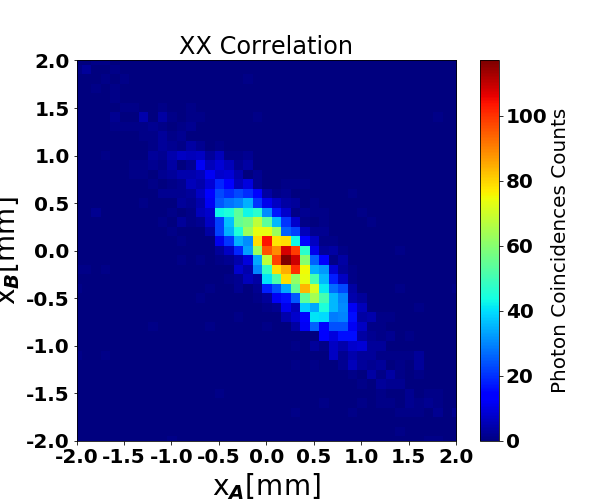
\includegraphics[width=0.45\textwidth]{Figures/xxCorrelation.png} }
{  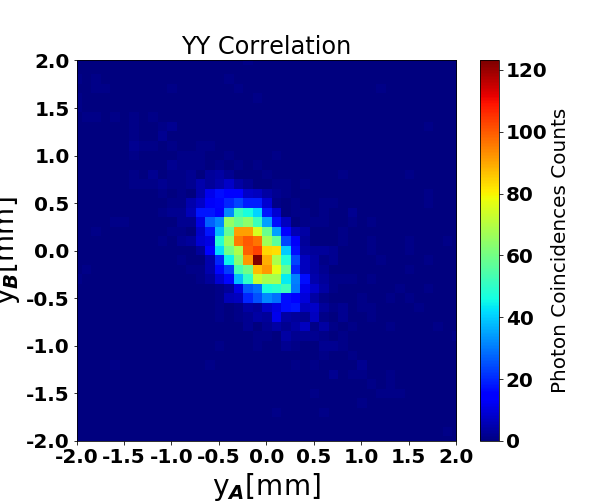
\includegraphics[width=0.45\textwidth]{Figures/yyCorrelation.png} }
\caption{Experimental Spatial correlations between a pair of down-converted photons. \textit{XX Correlation} shows the correlation in the x variables. \textit{YY Correlation} shows the correlation in the y variables, Beam propagating in the z direction. $w_p = 91\mu m$}
 \label{fig:expCorrelations}
\end{figure}

Figure \ref{fig:expCorrelations}(\textit{YY Correlation}) show the spatial correlation in 
the yy direction, this image is done by repeating the same recipe as before, but this 
time scanning and moving in the y direction.
The spatial correlations in this case present a negative behaviour in both XX and YY direction, an anticorrelation.
Meaning that is expected to measure a photon at a negative position at the B 
path if we measured a photon at a positive position at the A path. They both exhibit a elliptical
shape, but the XX correlation is a narrower one, meaning there is a stronger relation
between the pair of photons in the X direction.

\section{Mask Alignment}

Before making a Two-photon image we need to know that we have placed the mask in the correct 
spot. This correct spot is defined by the Figures \ref{fig:mask1} and \ref{fig:masks}. Which
localisation was decided in function of where the flux of correlated photon was greater.
The following images where produced as the standar image is done. It means we show the shadow
of the aperture in the B path. Every position of the images is the single 
counts of the $D_B$ in the exposure time. 

\subsection{Alignment Mask 1}
The Following Figure \ref{fig:localizationSq} shows the final localisation of the first
mask used. It was the final position because its position is really similar to the one described
in Figure \ref{fig:mask1}. For making this image we set the step length to be $0.2mm$ and
the exposure time was 1 second per position.

\begin{figure}[h!]
\centering
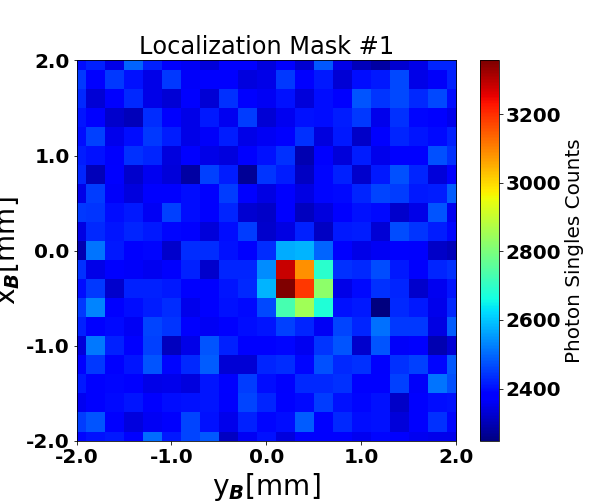
\includegraphics[width=0.6\textwidth]{Figures/localizationSq.png} 
\caption{Localization of the mask with an square}
\label{fig:localizationSq}
\end{figure}

\subsection{Alignment Mask 2}
Figure \ref{fig:localizationL} shows the localisation of the second mask. While in Figure \ref{fig:localizationL}(A)
there is the initial position of the mask, Figure \ref{fig:localizationL}(B) shows
the new localisation of the aperture after a translation in the y direction. This images
where done by setting the steps to $0.2mm$ and the exposure time to 1 second per position.


\begin{figure}[h!]
\centering
{  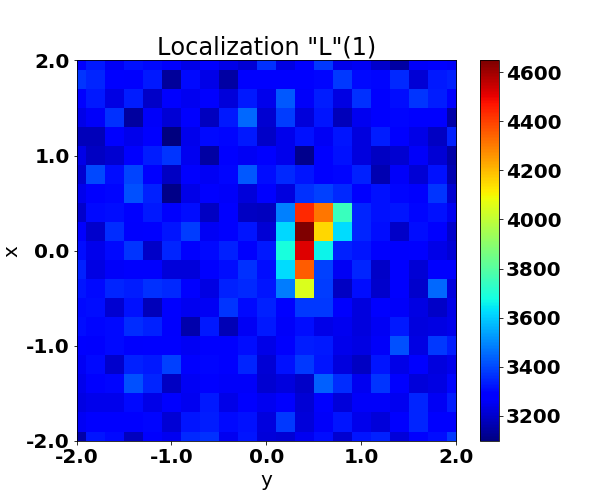
\includegraphics[width=0.45\textwidth]{Figures/localizationL1.png} }
{  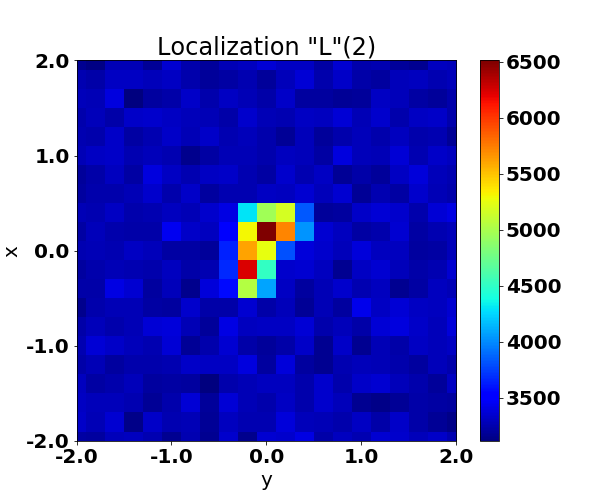
\includegraphics[width=0.45\textwidth]{Figures/localizationL2.png} }
\caption{Moving the L Mask in order to put it in the most central spot}
 \label{fig:localizationL}
\end{figure}
In Figure \ref{fig:localizationDef} is presented the definitive position of the aperture
before making a Two-photon imaging. If we take a closer look to the Figure, we can appreciate
a higer contrast, this is because in this opportunity we set the steps to be $0.1mm$ and 
the exposure time to be 30 seconds per position. This image is the result of measuring for around 
14 hours.
\begin{figure}[h!]
\centering
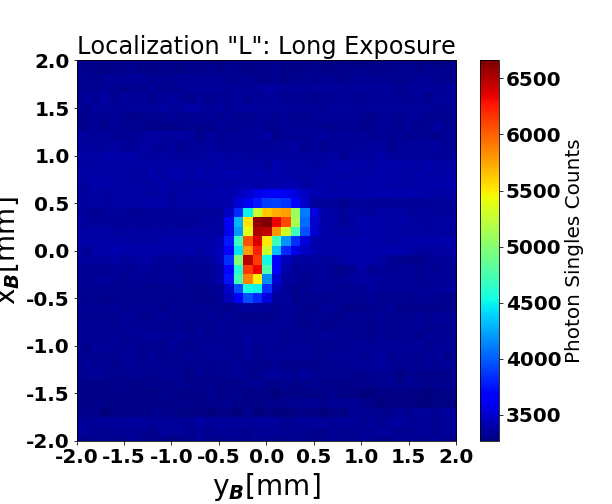
\includegraphics[width=0.6\textwidth]{Figures/localizationLLong.png} 
\caption{Long exposure of the definitive localization of the mask, in this try we leave the 
detector in each place for 30 seconds, we also make the steps of the detector smaller, $0.1mm$}
\label{fig:localizationDef}
\end{figure}
\subsection{Alignment Mask 3}

The definitive localisation of the third mask used is presented in the Figure \ref{fig:localizationInte}, 
where the step was $0.1mm$ and the exposure time was set to 30 seconds per position.

\begin{figure}[h!]
\centering
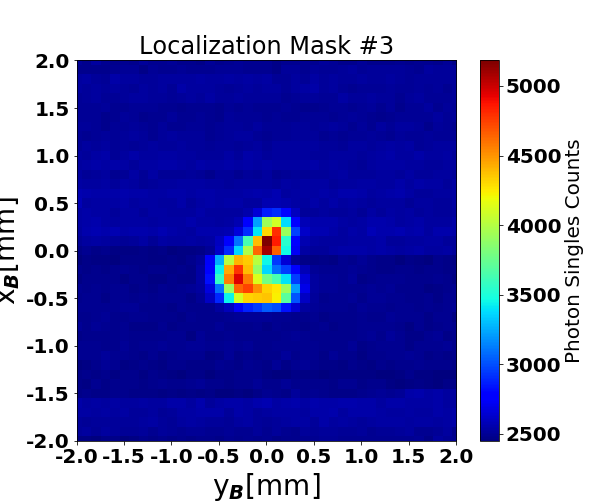
\includegraphics[width=0.6\textwidth]{Figures/interrogationLocation.png} 
\caption{Interrogation definitive position}
\label{fig:localizationInte}
\end{figure}


\section{Two-Photon Images}

Finally we get to observe the Two-photon images that are the core of this monograh,
It is important to remember the way this images are obtained. The image $R(\vec{r}_A)$ is a 
function of the coincidence counts between $D_C$ and $D_A$. We scan $D_A$, and as a 
result we obtain a 2-D matrix where each ($i,j$) position is the coincidence counts.

\subsection{Two-photon imaging Mask 1}

Figure \ref{fig:twoPhotonSq} is the Two-photon image of the square aperture. The maximun
coincidence counts changed position in the image, compared to Figure \ref{fig:localizationSq}.
The shape is not identificable,  and its position
is reflected in both x and y direction, as an evidence of the anticorrelations we are using Figure \ref{fig:expCorrelations} 
\begin{figure}[h!]
\centering
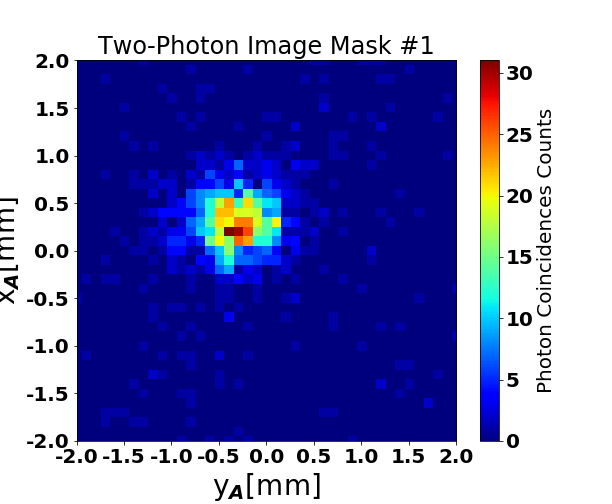
\includegraphics[width=0.6\textwidth]{Figures/two-photonImageSq.png} 
\caption{Experimental Two-photon image recovered for the square aperture}
\label{fig:twoPhotonSq}
\end{figure}

\subsection{Two-photon imaging Mask 2}
The Two-photon image of the second mask is presented in Figure \ref{fig:twoPhotonL}. 
In this opportunity it is clear that the more complex shape of the aperture is hardly
identifiable. However, there are some other interesting things to note about the image.
As the original aperture, the image is not symmetrical, and it is not pointing to the
original direction the L was in Figure \ref{fig:mask2}. This make us to think 
about reflexions in the image respect from the original mask, but in this case is 
not that easy to detect.
\begin{figure}[h!]
\centering
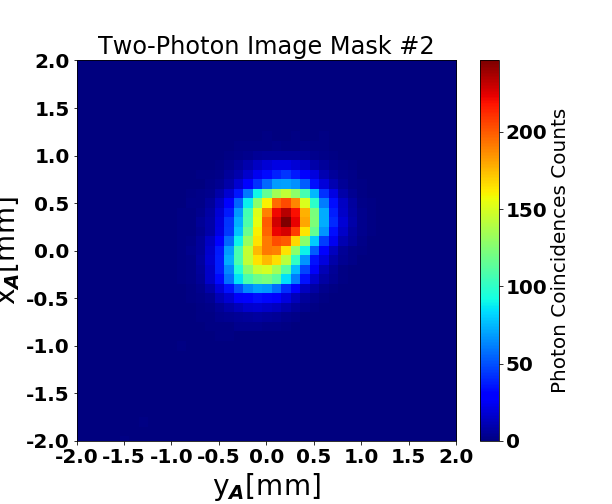
\includegraphics[width=0.6\textwidth]{Figures/twoPhoL.png} 
\caption{Two-photon image recovered for the L aperture.}
\label{fig:twoPhotonL}
\end{figure}



\subsection{Two-photon imaging Mask 3}
The third Two-photon image is in Figure \ref{fig:twoPhotonInte}. Again the complex original
shape is barely visible in the image obtained, Nevertheless this result and the other Two-photon image is
really instructive about what we can expect with different spatial correlations. The step for this Figure was $0.01mm$ and the exposure time 
was of 30 seconds per position. 
\begin{figure}[h!]
\centering
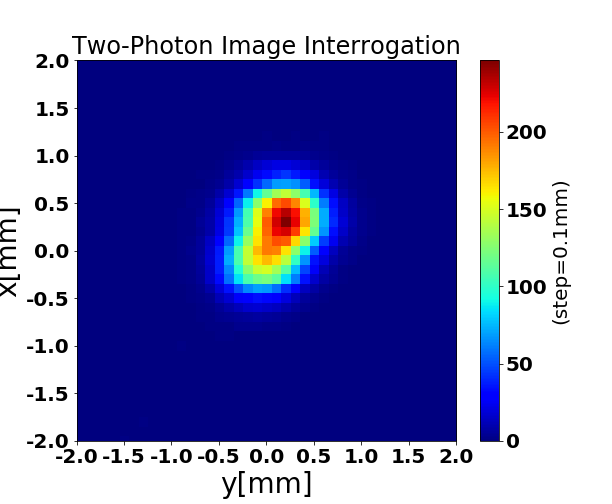
\includegraphics[width=0.6\textwidth]{Figures/twoPhotonInte.png} 
\caption{Two-Photon Image Interrogation}
\label{fig:twoPhotonInte}
\end{figure}

